\documentclass{article}
\usepackage[utf8]{inputenc}
% Globally defined colors
\usepackage{xcolor}
\definecolor{alternateKeywordsColor}{rgb}{0.13,1,0.13}
\definecolor{keywordsColor}{rgb}{0.13,0.13,1}
\definecolor{commentsColor}{rgb}{0,0.5,0}
\definecolor{stringsColor}{rgb}{0,0,0.5}
\usepackage{listings}
\lstdefinelanguage{fsharp}{%
  keywords={abstract, and, as, assert, base, begin, class, default, delegate, do, done, downcast, downto, elif, else, end, exception, extern, false, finally, for, fun, function, global, if, in, inherit, inline, interface, internal, lazy, let, match, member, module, mutable, namespace, new, null, of, open, or, override, private, public, rec, return, sig, static, struct, then, to, true, try, type, upcast, use, val, void, when, while, with, yield},
  morekeywords={atomic, break, checked, component, const, constraint, constructor, continue, eager, fixed, fori, functor, include, measure, method, mixin, object, parallel, params, process, protected, pure, recursive, sealed, tailcall, trait, virtual, volatile},
  otherkeywords={ let!, return!, do!, yield!, use!},
  keywordstyle=\color{keywordsColor},
  % sensitive=true,
  basicstyle=\ttfamily\lst@ifdisplaystyle\footnotesize\fi, % make font small for listings but not for lstinline
  breaklines=true,
  breakatwhitespace=true
  showstringspaces=false,
  morecomment=[l][\color{commentsColor}]{///},
  morecomment=[l][\color{commentsColor}]{//},
  morecomment=[n][\color{commentsColor}]{(*}{*)},
  morecomment=[is][\color{white}]{(*//}{*)},
  morestring=[b]",
  literate={`}{\`}1,
  stringstyle=\color{stringsColor},
  showspaces=false,
  numbers=left,
  numbersep=1.5pt,
  numberstyle=\scriptsize\color{white},
  % aboveskip=0pt, 
  % belowskip=0pt,
  % resetmargins=true,
  % captionpos=b,
  backgroundcolor=\color{black!5!white},
}
\lstset{language=fsharp}
\usepackage{comment}
\usepackage{graphicx}
\graphicspath{ {./figs/} }
\usepackage[noabbrev,capitalize]{cleveref}

\title{Canvas}
\author{Jon Sporring}
\date{August 2022}

\begin{document}

\maketitle

\section{Introduction}
Canvas is a small F\# library by which you can open a window and manipulates its pixels. In the following, we will describe how to write a simple graphics application. Consider the following example:
\begin{lstlisting}
#r "nuget:DIKU.Canvas, 1.0.0-alpha2"

open Canvas

let w = 600;
let h = 400;
let C = create w h
do setLine C black (0,0) (w-1,h-1)
do show C "My First Canvas"
\end{lstlisting}
Saving the above in a file \texttt{myFirstCanvas.fsx} and running it with \texttt{dotnet fsi myFirst} in the terminal, should create a window on the screen with a black line going diagonally from the top left to the bottom right shown in \Cref{fig:myFirstCanvas}.
\begin{figure}
  \centering
  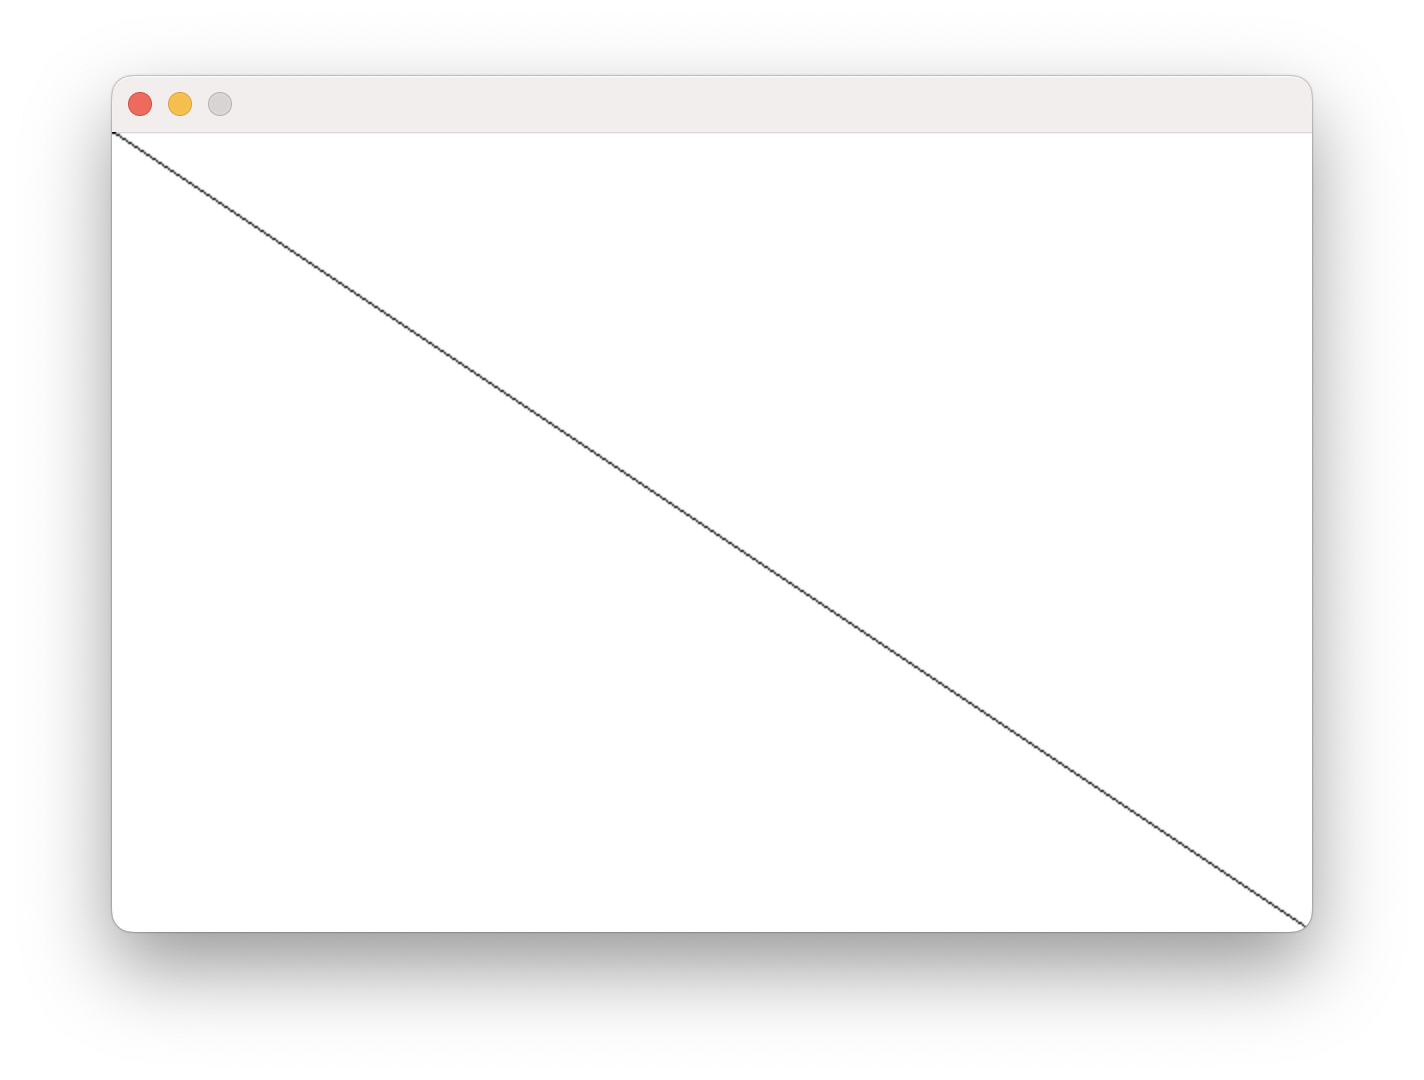
\includegraphics[width=0.45\textwidth]{myFirstCanvas}
  \caption{A demonstration of the output of Canvas.}
  \label{fig:myFirstCanvas}
\end{figure}
The program terminates, when you close the window or press \texttt{<ctrl-c>} in the terminal. The program first creates a canvas with the \lstinline{create}, then it draws a line on the canvas with \lstinline{setLine}, and finally, it shows the canvas on the screen, i.e., it tells the operating system to open a window and display the canvas.

\section{Drawing in canvas}
A canvas is a 2-dimensional buffer that stores pixels, and it is created using the function,
\begin{lstlisting}
create : int -> int -> canvas
\end{lstlisting}
It takes a width and a height and returns a canvas. It has an integer coordinate system, whose origin is in the top left corner, the first coordinate increases to the right, and the second coordinate increases downwards I.e., for a canvas with width and height $(w,h)$ then a canvas coordinate $(i,j)$ has $0\leq i < w$ and $0\leq j < h$, such that $(0,0)$ is the top-left corner and $(w-1,h-1)$ is the bottom-right corner. For a given canvas, its width and height can be obtained with the functions,
\begin{lstlisting}
width       : canvas -> int
height      : canvas -> int
\end{lstlisting}

Each pixel is a combination of 4 values: red, green, blue, and alpha, also known as RGBA. Each value is an unsigned, 8-bit integer, the red-green-blue in combination gives represents all the colors, the screen can display, and alpha is the degree of transparency, such that $(r,g,b,a) = (255,0,0,255)$ is a red and non-transparent pixel, and $(r,g,b,a) = (0,255,0,128)$ is a semi-transparent green pixel. You can manipulate colors with 
\begin{lstlisting}
fromRgb   : int * int * int -> color
fromArgb  : int * int * int * int -> color
fromColor : color -> int * int * int * int
\end{lstlisting}
and there are a number of builtin colors: \lstinline{red}, \lstinline{blue}, \lstinline{green}, \lstinline{yellow}, \lstinline{lightgrey}, \lstinline{white}, and \lstinline{black}.

The value of a pixel can be read using
\begin{lstlisting}
getPixel    : canvas -> int * int -> color
\end{lstlisting}
which is a pixel that takes an existing canvas and a coordinate pair (2-tuple) and returns the pixel's color.
To write a pixel, use
\begin{lstlisting}
setPixel    : canvas -> color -> int * int -> unit
\end{lstlisting}
Note that this function has a side effect! It takes a canvas, a color, and a coordinate pair and updates the canvas. Extensions of \lstinline{setPixel} are available for drawing lines and boxes:
\begin{lstlisting}
setLine     : canvas -> color -> int * int -> int * int -> unit
setBox      : canvas -> color -> int * int -> int * int -> unit
setFillBox  : canvas -> color -> int * int -> int * int -> unit
\end{lstlisting}
Again, these functions have the side-effect that the canvas is updated. They all take a canvas, a color, and two coordinate pairs. Assuming the coordinate pairs are \lstinline{p1} and \lstinline{p2}, then \lstinline{setLine} draws 
a line from \lstinline{p1} to \lstinline{p2}, \lstinline{setBox} draws the contour of a box, where \lstinline{p1} is the top left corner and \lstinline{p2} is the bottom right corner. The function \lstinline{setFillBox} draws a filled box with \lstinline{p1} and \lstinline{p2} being its corners.

Manipulating pixels only manipulates an internal representation of the canvas but does not change anything on the screen. When the canvas has been drawn upon, it can be shown with
\begin{lstlisting}
show      : canvas -> string -> unit
\end{lstlisting}
which takes a canvas and a title string, and opens a window that displays the canvas. The function returns when the user closes the window. It can also be stopped by pressing \texttt{<ctrl-c>}.

\section{Turtle graphics}
Turtle graphics is an alternative method of drawing line drawings in canvas. The turtle is a metaphor for a small animal, which can do simple actions, and in Canvas the turtle can turn and move with \lstinline{Turn}, \lstinline{Move}, and left the pen up and down with \lstinline{PenUp} and \lstinline{PenDown}. The turtle starts in the center of the screen pointing upwards. An example of a turtle program is as follows:
\begin{lstlisting}
#r "nuget:DIKU.Canvas, 1.0.0-alpha2"

open Canvas

let cmd = [Move 100; Turn 90; Move 200]
let w = 600;
let h = 400;
do turtleDraw (w,h) "My First Canvas" cmd
\end{lstlisting}
This should produce a window as shown in \Cref{fig:myFirstTurtle}.
\begin{figure}
  \centering
  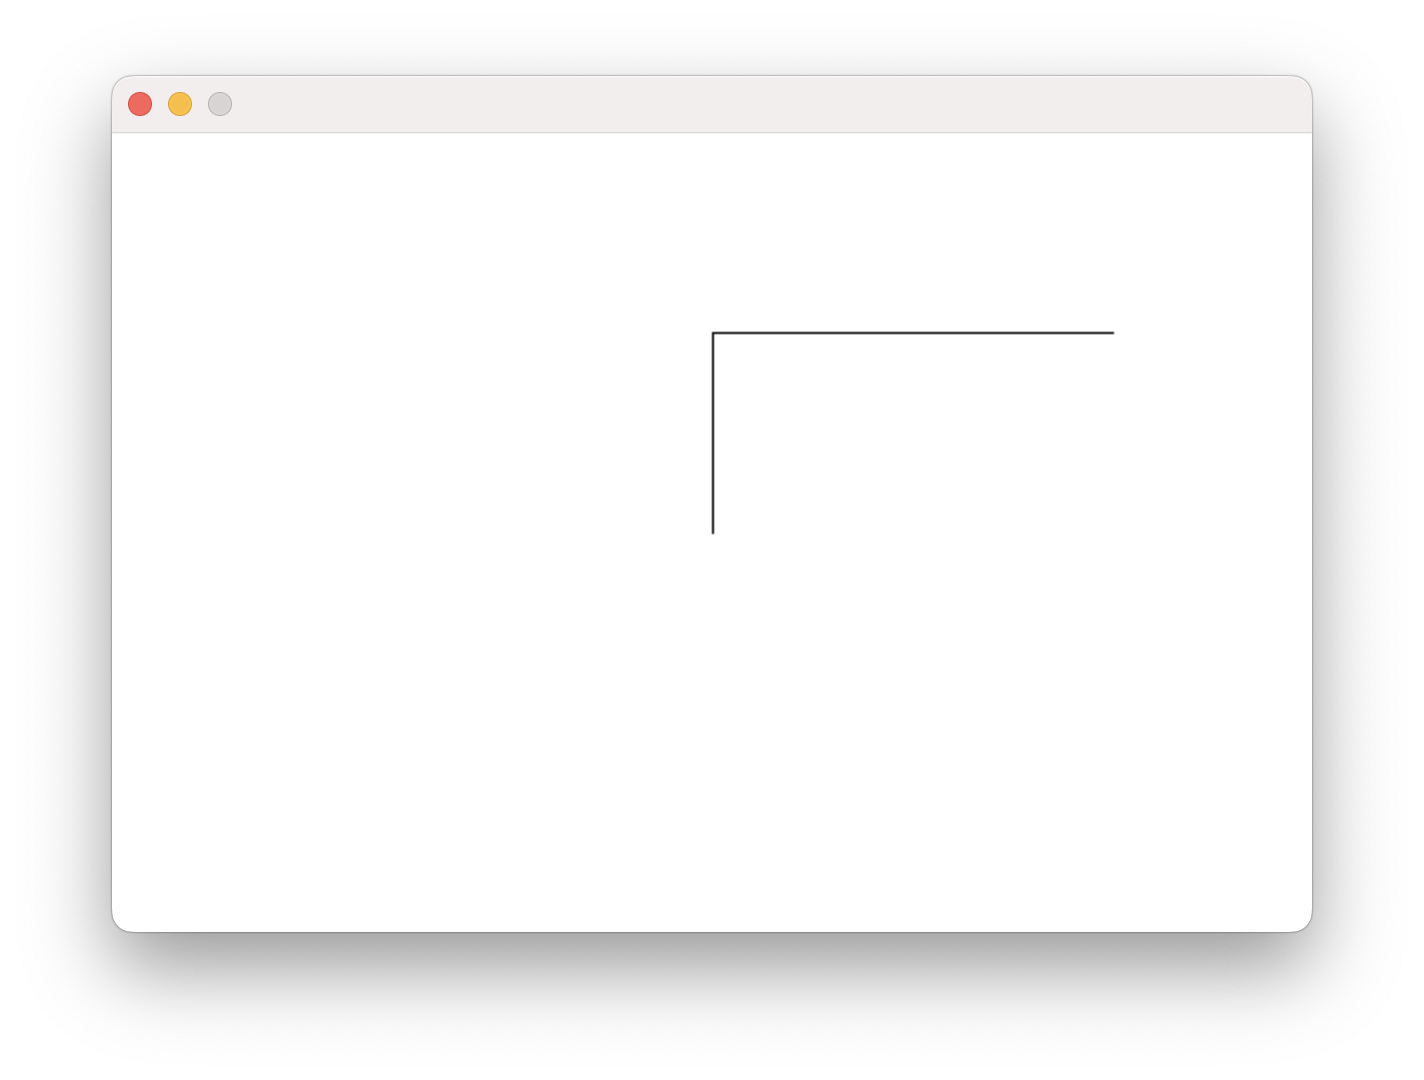
\includegraphics[width=0.45\textwidth]{myFirstTurtle}
  \caption{A demonstration of turtle graphics in Canvas.}
  \label{fig:myFirstTurtle}
\end{figure}
The commands are given as a list of \lstinline{turtleCmd}, which can be one of either
\begin{lstlisting}
SetColor of color
Turn of int
Move of int
PenUp
PenDown
\end{lstlisting}
The SetColor is used to set a color, e.g., \lstinline{SetColor green} will make the next line, the turtle draws, green. Turning the turtle is done in degrees, e.g., \lstinline{Turn 30} will make the turtle point in a new direction which is 30 degrees clockwise turn compared to the present direction.  \lstinline{Move 15} will make the turtle move 15 pixels in the direction, it is pointing. If the pen is down, as it is per default, then it will also draw a line on its path. \lstinline{PenUp} and \lstinline{PenDown} lowers or raises the pen. The turtle's starting point is the center of the Canvas pointing up, with a black pen down. The commands are given as a list, i.e.,  elements are separated by semicolons, and the commands are executed from left to right. The function
\begin{lstlisting}
turtleDraw : int*int -> string -> turtleCmd list -> unit
\end{lstlisting}
makes a canvas with a list of commands. \lstinline{turtleDraw} takes a width-height pair, the name of a window, and the list of commands, and opens a window on the screen. The function returns, once the window is closed by the user. 

\section{Interaction with the user}
Canvas can be programmed to respond to user input by listining to the keyboard. To do this, we use \lstinline{runApp} instead of \lstinline{show}. The function \lstinline{runApp} has the following interface:
\begin{lstlisting}
// start an app that can listen to key-events
runApp    : string -> int -> int
             -> (int -> int -> 's -> canvas)
             -> ('s -> key -> 's option)
             -> 's -> unit
\end{lstlisting}
It takes a window title as a string, a width and a height, a function that can draw a create a canvas with content, and a function that can listen and react to keyboard input and a state. Consider the following example:
\begin{lstlisting}
#r "nuget:DIKU.Canvas, 1.0.0-alpha2"

open Canvas

type state = color

let draw w h (s:state) =
  let C = Canvas.create w h
  setFillBox C s (0,0) (w-1,h-1)
  C

let react (s:state) (k:Canvas.key) : state option =
    match getKey k with
        | LeftArrow ->
            printfn "Going red!"
            Some red
        | RightArrow ->
            printfn "Going blue!"
            Some blue
        | _ -> None

do runApp "ColorTest" 600 600 draw react red
\end{lstlisting}
When the program is run, it opens a window and paints everything inside it red. When the user presses the right arrow key, the screen is painted blue, and ``Going blue!'' is printed on the terminal, and when the left arrow key is pressed, then the screen is painted red, and ``Going red!'' is printed in the terminal. The program is stopped by closing the window or pressing \texttt{<ctrl-c>}.

The program works as follows: \lstinline{runApp} maintains an internal state, whose type is defined by the user. Here \lstinline{state} can be defined to be anything but here it is a color. Let us call this \lstinline{s}. The initial value of this state is set by \lstinline{runApp}'s last argument, here \lstinline{red}. After the state has been initialized, \lstinline{runApp} calls \lstinline{draw w h s}, i.e., \lstinline{draw 600 600 red}, a window is created, and the canvas is shown on the screen. Then it waits for the user to press any key. The result is put in internal \lstinline{key}-value, let us call it \lstinline{k}, and \lstinline{runApp} calls the user-specified \lstinline{react} function with \lstinline{react s k}. This function must return an \lstinline{option} type, i.e., either \lstinline{Some t}, where \lstinline{t} is any state, or \lstinline{None}. If \lstinline{react} returns \lstinline{None}, then nothing happens. However, if \lstinline{react} returns \lstinline{Some t}, then \lstinline{runApp}'s internal state is changed to \lstinline{t}, \lstinline{draw} is called again but now with \lstinline{t} as the state, and the window's content is updated with the new canvas. To help all of this, the function
\begin{lstlisting}
getKey : key -> ImgUtilKey
\end{lstlisting}
converts the internal key-value to one of \lstinline{Unknown}, \lstinline{DownArrow}, \lstinline{UpArrow}, \lstinline{LeftArrow}, \lstinline{RightArrow}, and \lstinline{Space}.
\end{document}
